\section{Data-driven results}
In this section we present the results of the data-driven models.
We start by showing the numerical solution of the shallow water equations, then we present the predictions of the FNN and FNO models.
Until now, we have mostly considered discountinuous initial conditions, but we will also consider smooth initial conditions in this section.
We solve the SWE with the following initial conditions:
\begin{equation}
    \begin{aligned}
        h(x, 0) &= h_0 \exp \left( \frac{-{(x-\mu)}^2}{2 \sigma^2} \right) ,\\
        u(x, 0) &= 0 , \\
    \end{aligned}
\end{equation}
where $h_0 = 1, \mu = 0.5, \sigma = 0.1$. 
The domain is $ x \in [0, 1]$ with $N = 200$ points and the final time is $t = 1.0$.
We use a CFL number of $0.9$ and variable time steps.
The numerical solution is shown in Figure~\ref{fig:NN_initial}, in both a contour plot and a 3D plot.
\begin{figure}[H]
    \centering
    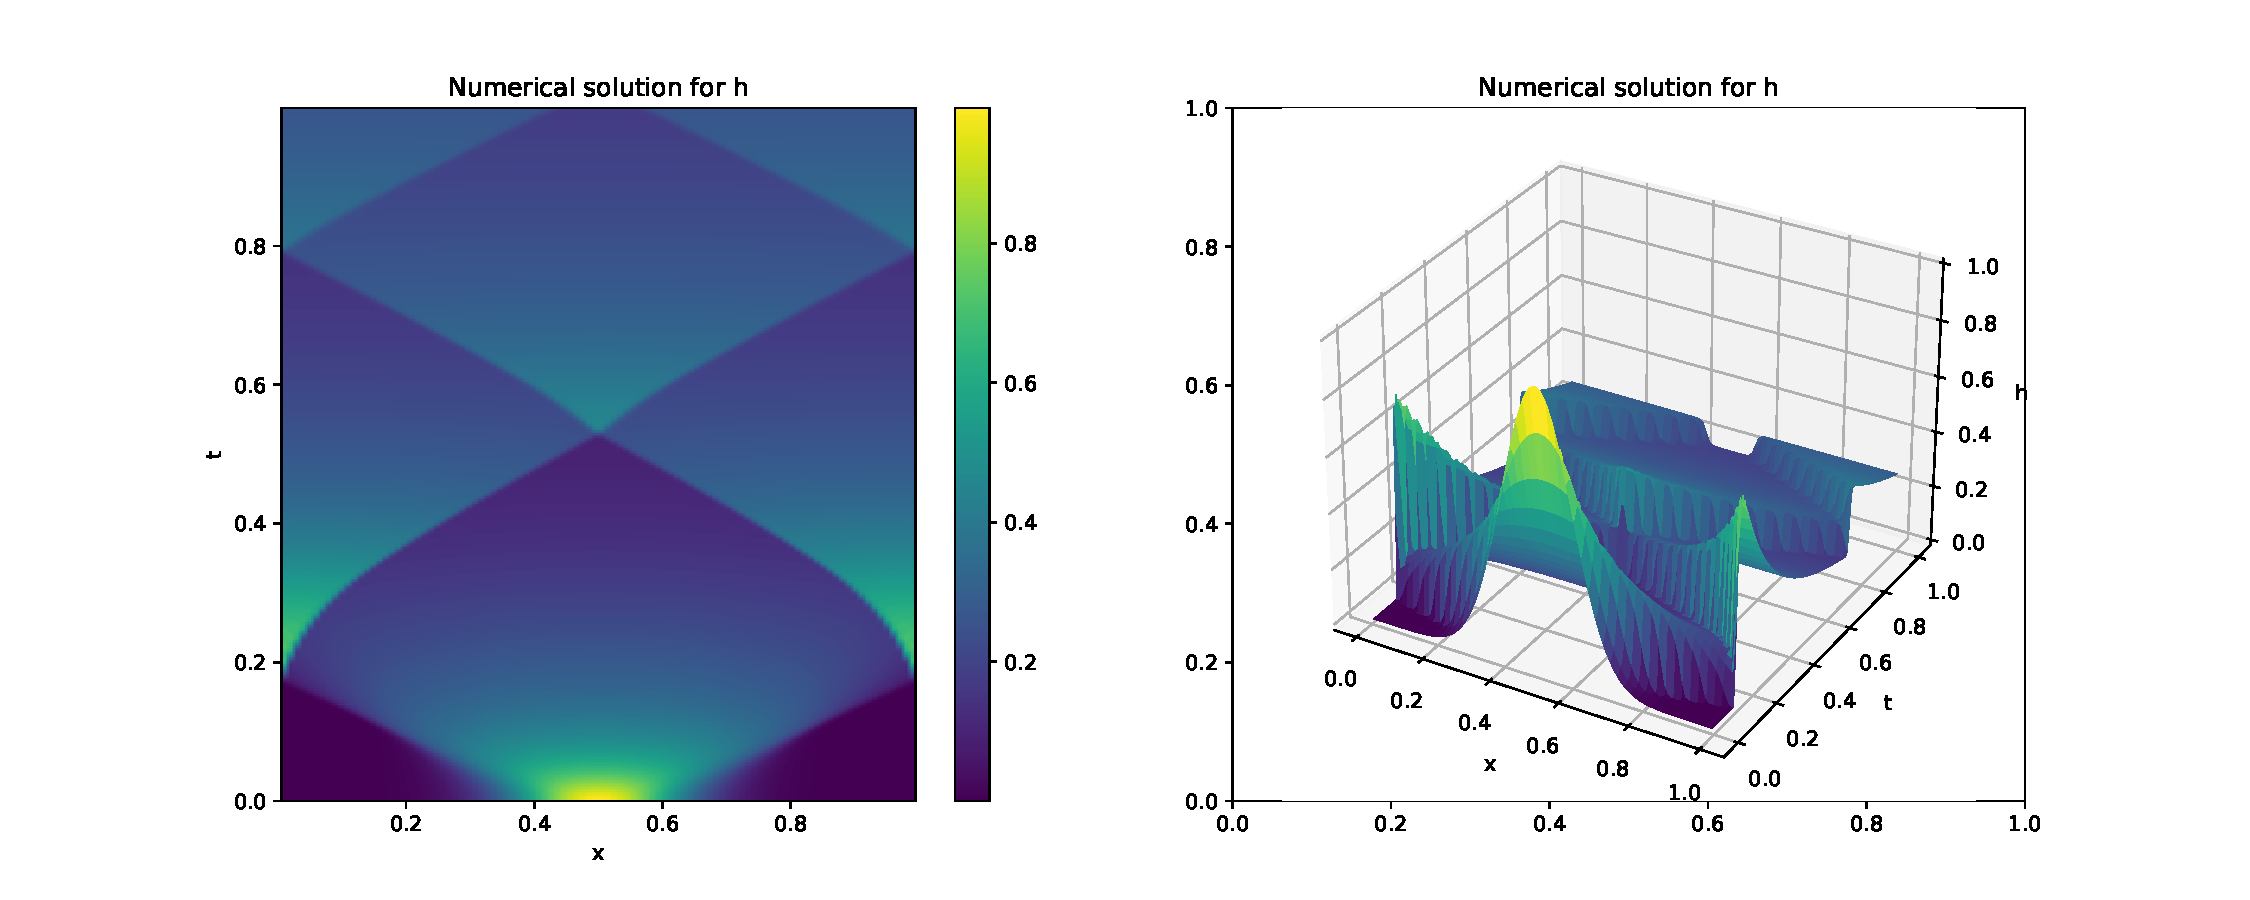
\includegraphics[width=0.7\textwidth]{C:/Users/Matteo/Shallow-Water-Equations/plots/NN_initial.pdf}
    \caption{Numerical solution of the shallow water equations.}\label{fig:NN_initial}
\end{figure}


\subsection{FNN}
In the feedforward neural network, we train the model using the data generated by the numerical solution of the shallow water equations.
The neural network consists of the following layers: a input dense layer, three hidden dense layers with ReLU activation functions, a batch normalization layer for stability, a dropout layer to prevent overfitting, and an output dense layer.
We have also included L2 regularization in the hidden layers to prevent overfitting.
Themodel has been trained using the Adam optimizer with a learning rate of $0.01$, a batch size of $16$ and a total of $3000$ epochs.
We train the model on the data from $t = 0$ to $t = 0.8$, and test it on the data from $t = 0.8$ to $t = 1.0$.
The predictions of the model are shown in \autoref{fig:NN_predictions}.

\begin{figure}[H]
    \centering
    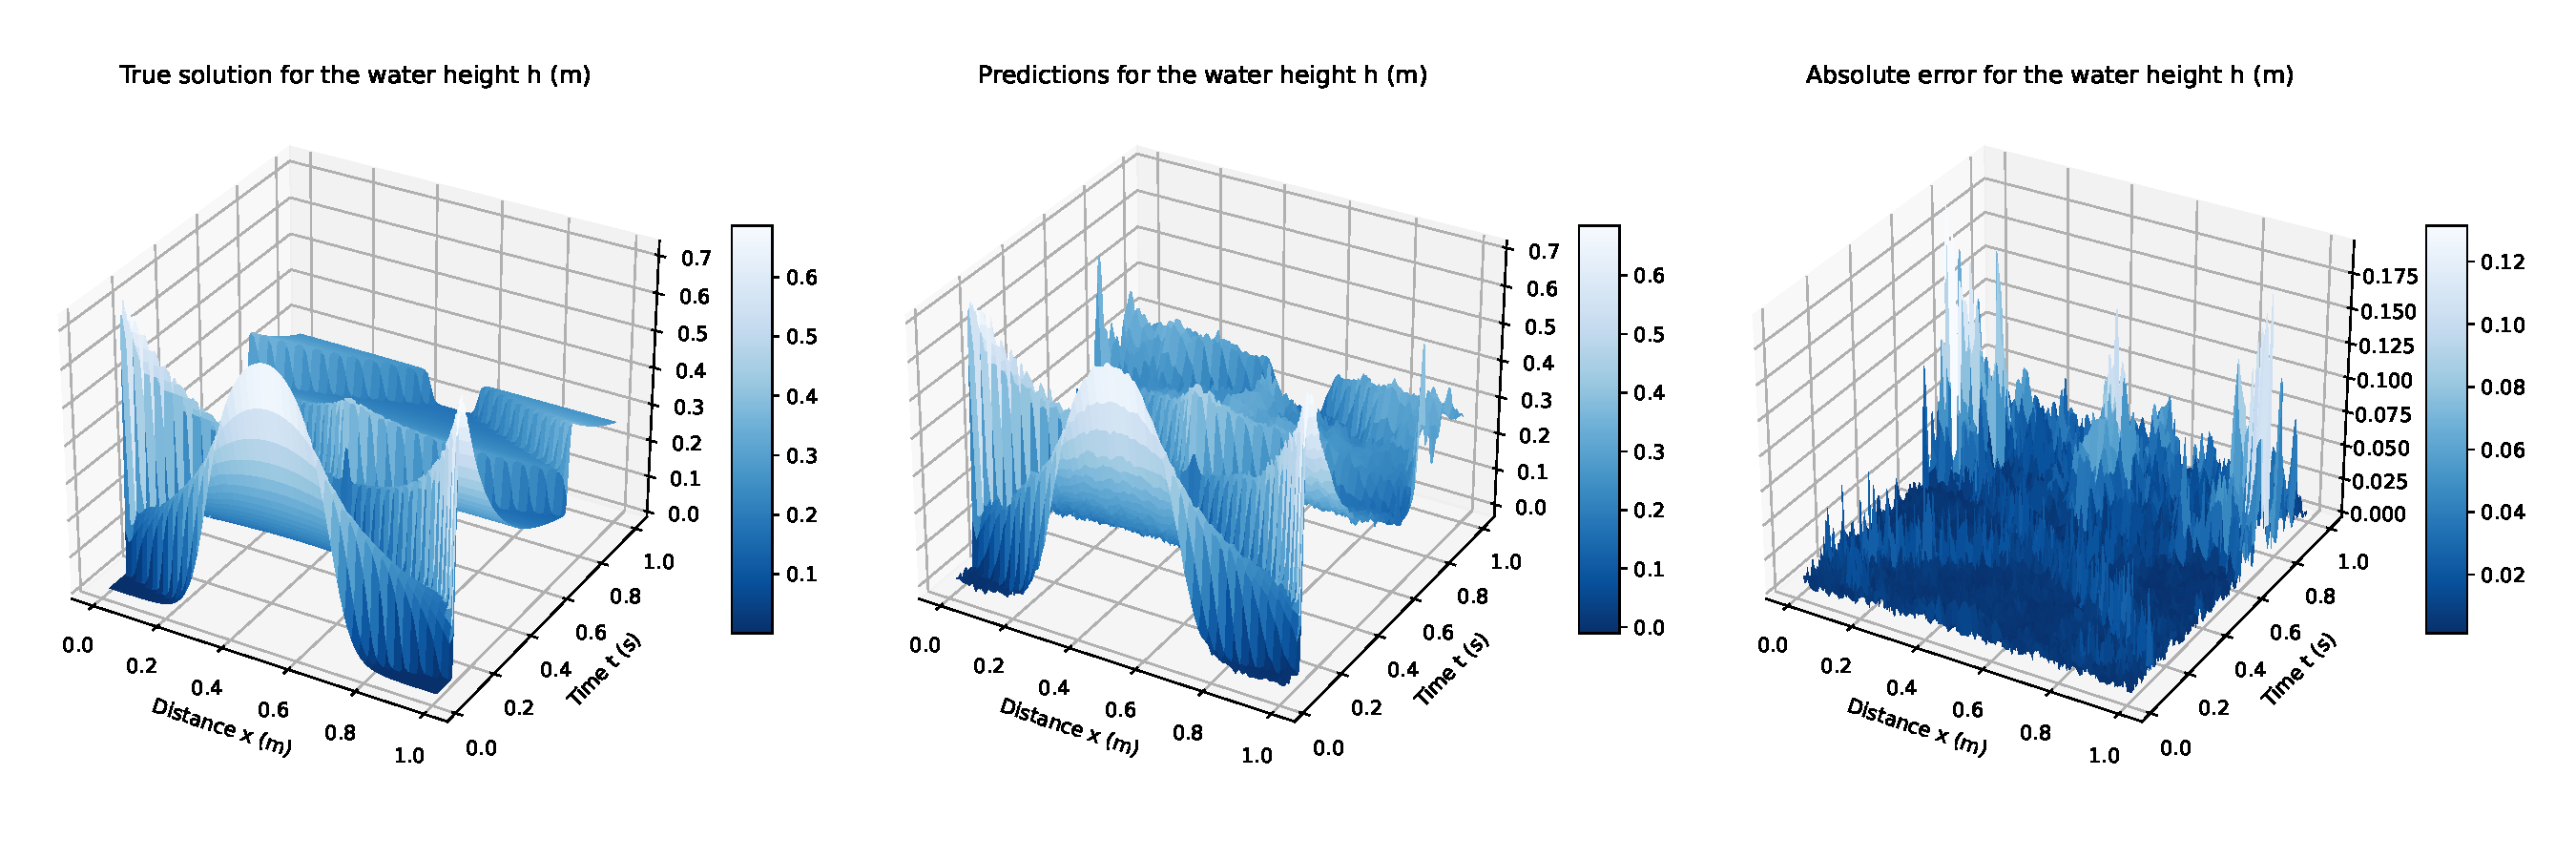
\includegraphics[width=0.99\textwidth]{C:/Users/Matteo/Shallow-Water-Equations/plots/NN_predictions.pdf}
    \caption{Predictions.}\label{fig:NN_predictions}
\end{figure}
From \autoref{fig:NN_predictions} we see that the neural network, to some extent, is able to learnt the dynamics of the solution, but it is not accurate enough to be used as a solver.
To understand the performance of the model, we consider the predictions for some given time steps, shown in \autoref{fig:NN_predictions_time_steps}.
\begin{figure}[H]
    \centering
    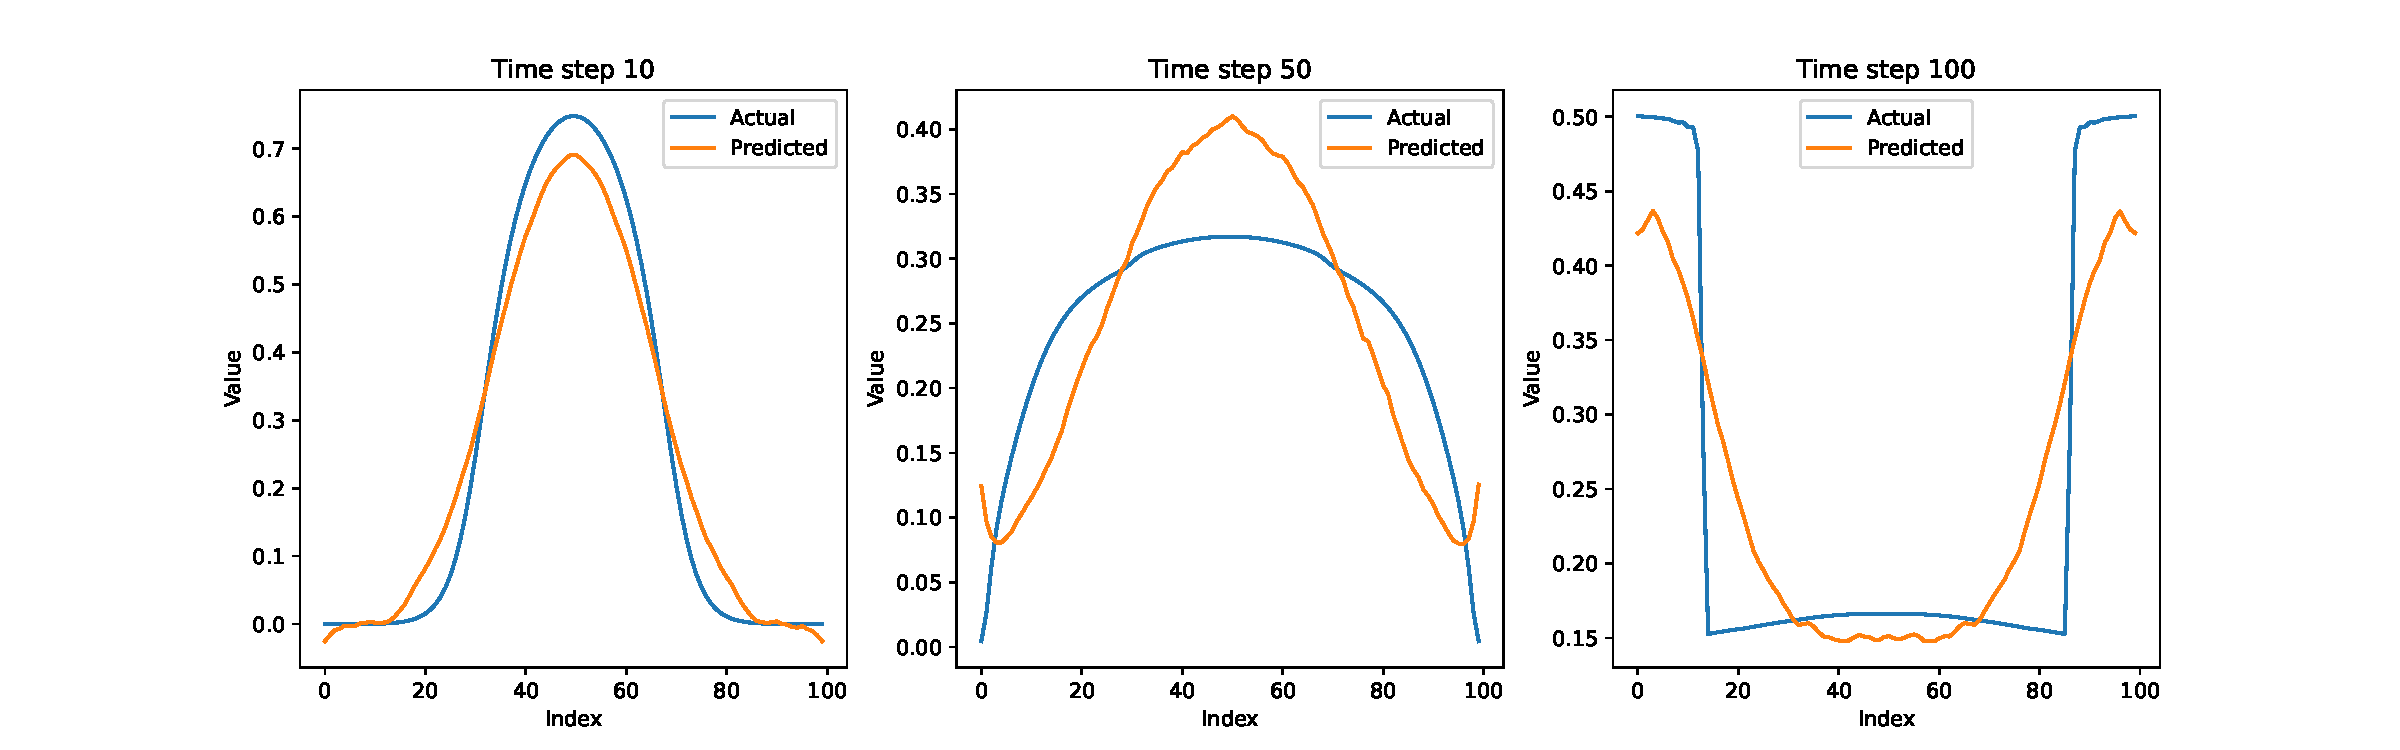
\includegraphics[width=0.95\textwidth]{C:/Users/Matteo/Shallow-Water-Equations/plots/NN_predictions_time_steps.pdf}
    \caption{Predictions for some given time steps.}\label{fig:NN_predictions_time_steps}
\end{figure}
Again, we see that the model finds some of the dynamics, but in practise, it can not be used as a solver.

The training and validation loss are shown in \autoref{fig:NN_loss_train_val}.
\begin{figure}[H]
    \centering
    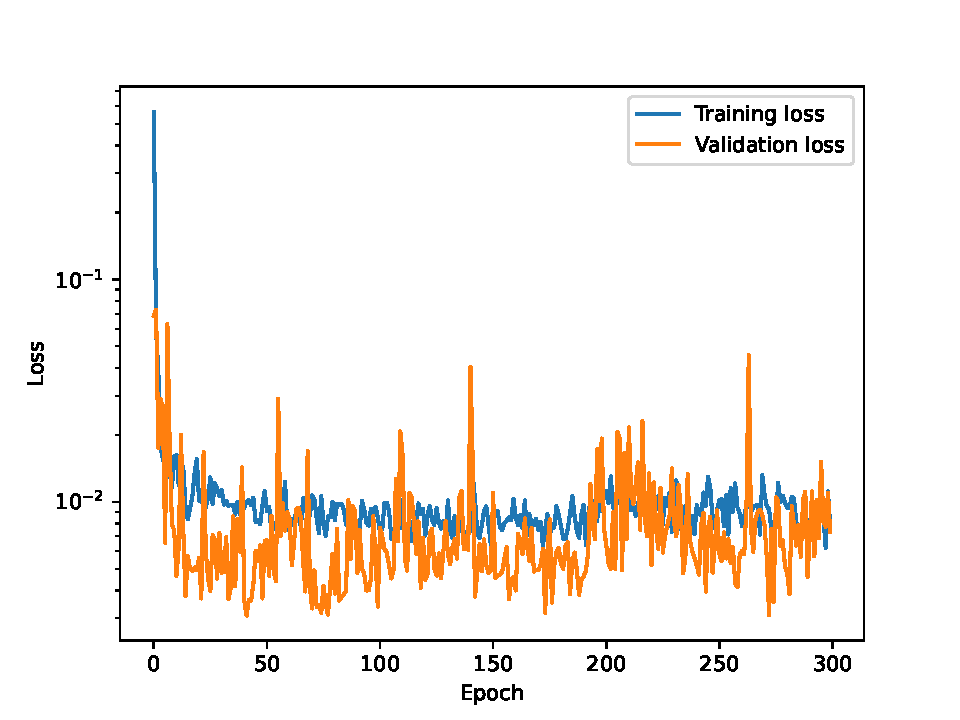
\includegraphics[width=0.6\textwidth]{C:/Users/Matteo/Shallow-Water-Equations/plots/NN_loss_train_val.pdf}
    \caption{Training and validation loss.}\label{fig:NN_loss_train_val}
\end{figure}
From \autoref{fig:NN_loss_train_val}, we see that a higher number of epochs, would probably not be beneficial, as the validation loss is increasing after a certain number of epochs.

We have also trained a LSTM model, but the results are not shown here, as the model was not able to learn the dynamics of the solution.



\subsection{FNO}
One of the main goals in this thesis is to use Fourier Neural Operators to solve the shallow water equations.
We define a FNO model, which consists of 2 input channels, 1 output channel, 100 Fourier modes in the first dimension and 1 Fourier mode in the second dimension.
The model is trained using the Adam optimizer with a learning rate of $0.001$, a total of $3000$ epochs and the critera is to minimize the mean squared error (MSE).
The results of the model are shown in \autoref{fig:FNO_predictions}.
\begin{figure}[H]
    \centering
    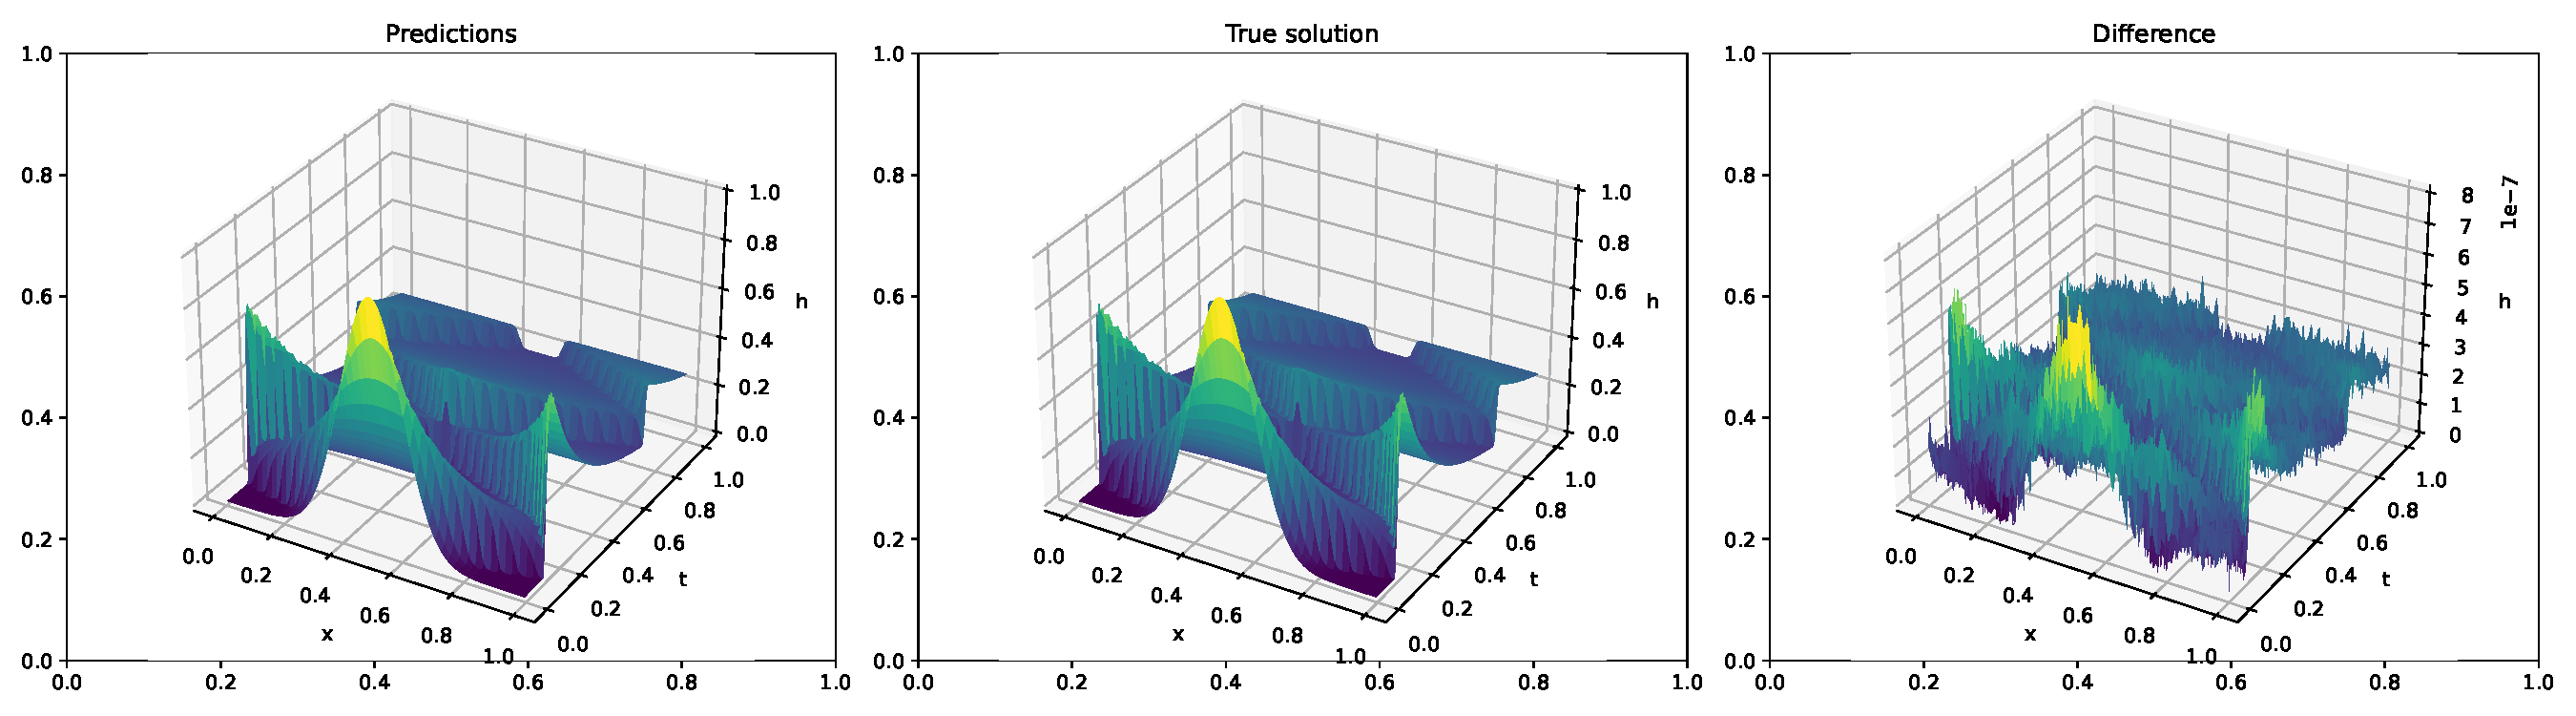
\includegraphics[width=0.95\textwidth]{C:/Users/Matteo/Shallow-Water-Equations/plots/FNOpredictions.pdf}
    \caption{FNO predictions.}\label{fig:FNO_predictions}
\end{figure}
From \autoref{fig:FNO_predictions} we see that the FNO model is able to learn the dynamics of the solution, and it is able to predict the solution with high accuracy.
The loss for each epoch is shown in \autoref{fig:FNO_loss}.
\begin{figure}[H]
    \centering
    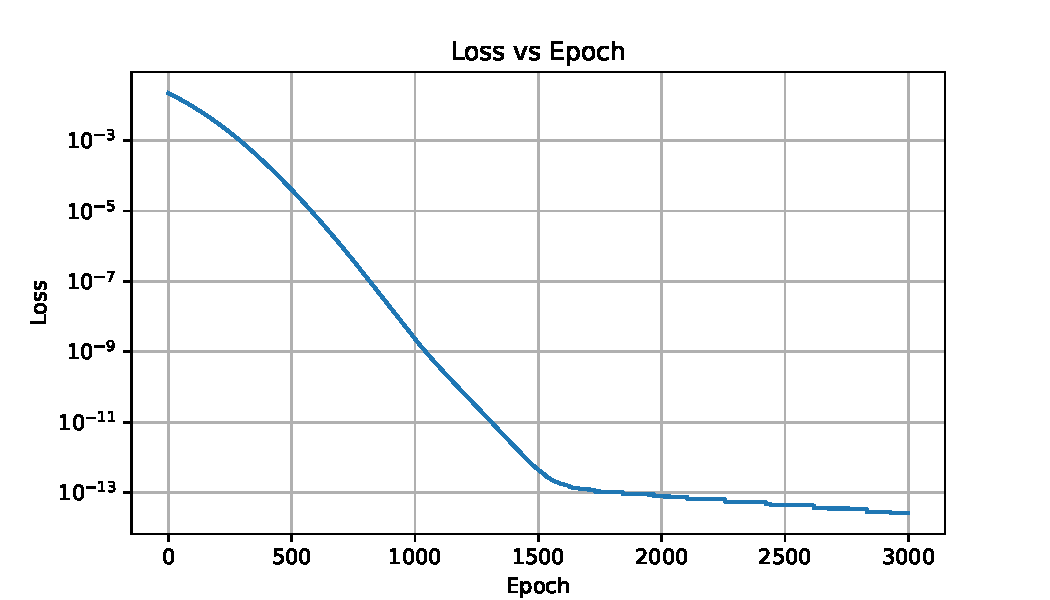
\includegraphics[width=0.5\textwidth]{C:/Users/Matteo/Shallow-Water-Equations/plots/FNOloss.pdf}
    \caption{FNO loss.}\label{fig:FNO_loss}
\end{figure}
From \autoref{fig:FNO_loss} we see that the loss is decreasing for each epoch, and the model is able to learn the dynamics of the solution.


